\section{Overview of the Approach}
\label{sec:overview}

The primary goal of our proposal is to provide a scalable architecture for executing incremental queries over large models.  Our approach is based on the following foundations: (i) a distributed model storage system that (ii) supports a graph-oriented data representation format, and (iii) a graph query language (adapted from the \incquery{} framework). The novel contribution of this paper is an architecture that consists of a (i) distributed model management middleware, and a (ii) distributed and stateful pattern matcher network based on the Rete algorithm. \incqueryD{} provides incremental query execution by \emph{indexing model contents} and \emph{capturing model manipulation operations} in the middleware layer, and \emph{propagating change tokens} along the pattern matcher network to \emph{produce query results and query result changes} (corresponding to model manipulation transactions) efficiently. As the primary sources of memory consumption, i.e.\ both the indexing and intermediate Rete nodes can be distributed in a cloud infrastructure, the system is expected to scale well beyond the limitations of the traditional single workstation setup.

\subsection{Architecture}
\label{architecture}
The \incqueryD{} architecture in an example configuration scenario is shown in \autoref{fig:architecture}.

\begin{figure}[!t]
\begin{center}
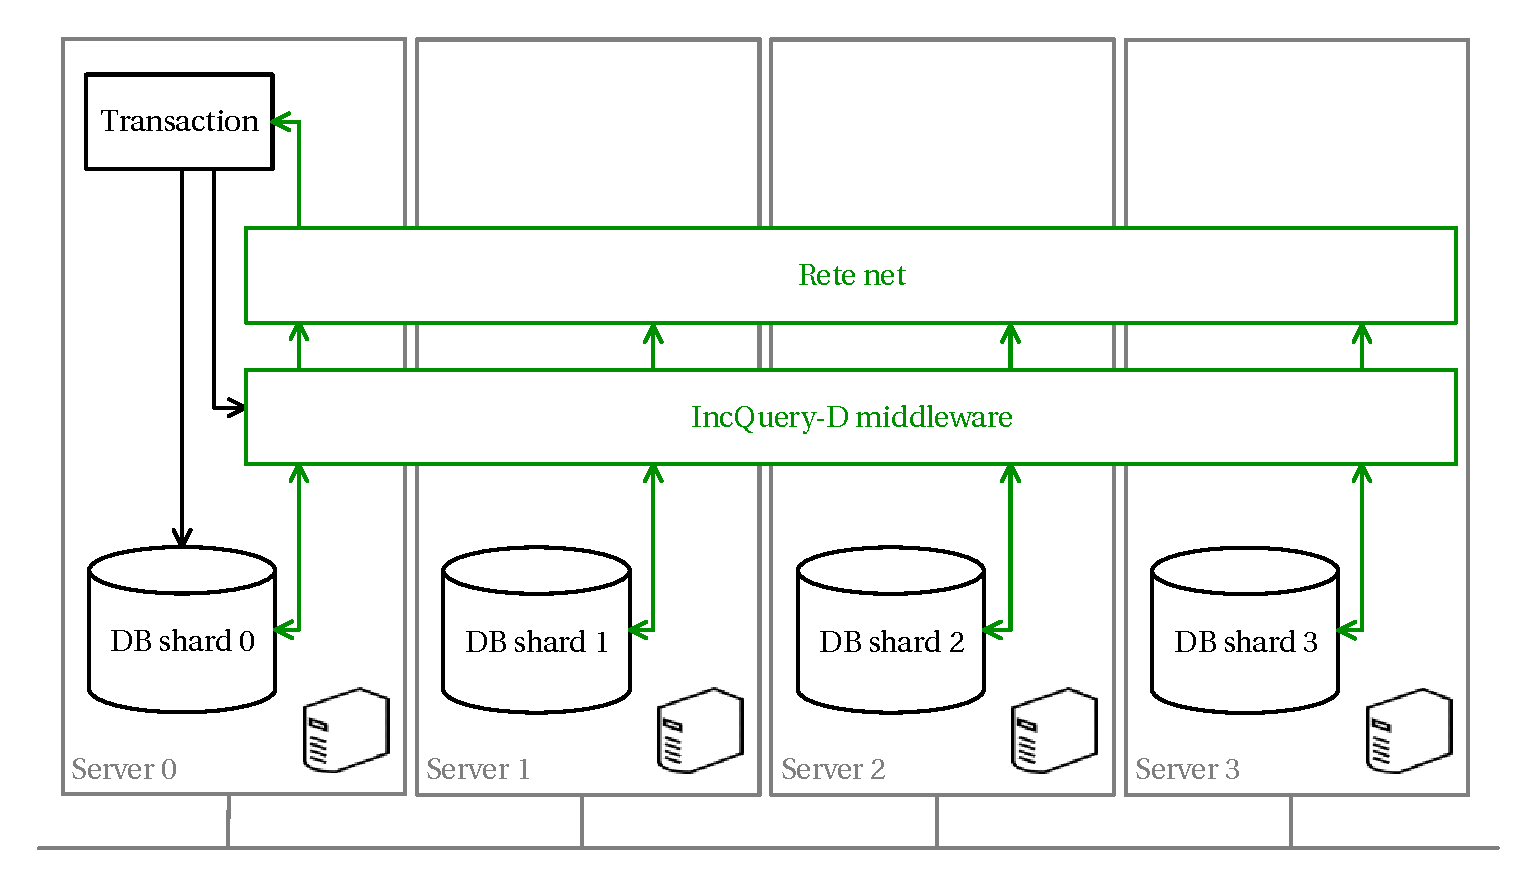
\includegraphics[width=.95\columnwidth]{figures/architecture}
\caption{A distributed, Rete-based model store and query system}
\label{fig:architecture}
\end{center}
\end{figure}


\emph{Storage and middleware.}\label{storage_and_middleware}
The proposed system is based on a distributed database management system.

In recent years, along long standing relational database management systems, dozens of new database systems sprung to life. This systems are often called NoSQL (short for not only SQL) databases.
These systems are often specialized to serve a specific aspect of Web 2.0 applications. To do so, they provide a non-relational data model and weaker consistency guarantees, but offer higher availability and better scalability.

In contrast to a traditional setup, where the distributed model repository (consisting of four shards in the example) is accessed on a per-node basis by a model manipulation transaction (such as a model transformation benchmark, depicted as $T_{BM}$ in \autoref{fig:architecture}), \incqueryD{} provides a middleware layer that offers three core services (shown in green in \autoref{fig:architecture}).
In {{\em distributed model management}}, the primary task is to provide a \emph{surrogate key} mechanism so that each model element in the entire distributed repository can be uniquely identified, and located within storage shards.
{{\em Model indexing}} is the key to high performance model queries. As MDE primarily uses a metamodeling infrastructure, the \incqueryD{} middleware maintains type-instance indexes so that all instances of a given type (both edges and graph nodes) can be enumerated quickly.
Finally, {{\em model change notifications}} are required by incremental query evaluation, thus model changes are captured and their effects propagated in the form of \emph{notification objects} (NOs). The middleware layer achieves this by providing a facade for model manipulation operations. 

Conceptually, the architecture of \incqueryD{} allows the usage of a wide scale of model representation formats. Our first prototype has been evaluated in the context of a low abstraction level \emph{property graph}~\cite{DBLP:journals/corr/abs-1006-2361} data model, but other mainstream metamodeling and knowledge representation languages such as Ecore~\cite{EMF} and RDF~\cite{website:rdf_standard} could be supported, as long as they can be mapped to an efficient and distributed storage backend (like key-value stores or column-family databases).


\emph{Distributed pattern matcher.}\label{distributed_pattern_matcher}
On top of the middleware, \incqueryD{} constructs a distributed and asynchronous network of communicating nodes that implement the Rete~\cite{Forgy} algorithm (shown within the dashed region in \autoref{fig:architecture}). This layer is essentially a dataflow network, with two types of nodes. Change notification objects (tokens) are propagated to intermediate \emph{worker nodes} that perform operations (like filtering tokens based on constant expressions, or performing join or antijoin operations based on their contents) and
store partial (interim) query results in their own memory. In contrast, \emph{production nodes} are terminators that provide an interface for fetching query results and also their changes. Connections between nodes can be \emph{local} (within one host) or \emph{remote} (when two Rete nodes are allocated to different hosts). It is important to emphasize that the database shards and Rete nodes are two distinct levels of distribution that do not directly depend upon each other.

\begin{figure}[!h]
\begin{center}
\begin{tabular}{cc}
\begin{minipage}{0.35\columnwidth}
\begin{lstlisting}
pattern test(
  V1:Type1, V2:Type2,
  V3:Type3, V4:Type4) {
  Type1.edgeType1(V1, V2);
  // join 1
  Type2.edgeType2(V2, V3);
  // join 2
  Type3.edgeType3(V3, V4);
  // antijoin 
  neg find anti(V4, V1); 
}
pattern anti(V4, V1) {
 Type1.edgeType4(V4, V1);
}
\end{lstlisting}
\end{minipage}
\hspace{0.5cm}
\begin{minipage}{0.45\columnwidth}
  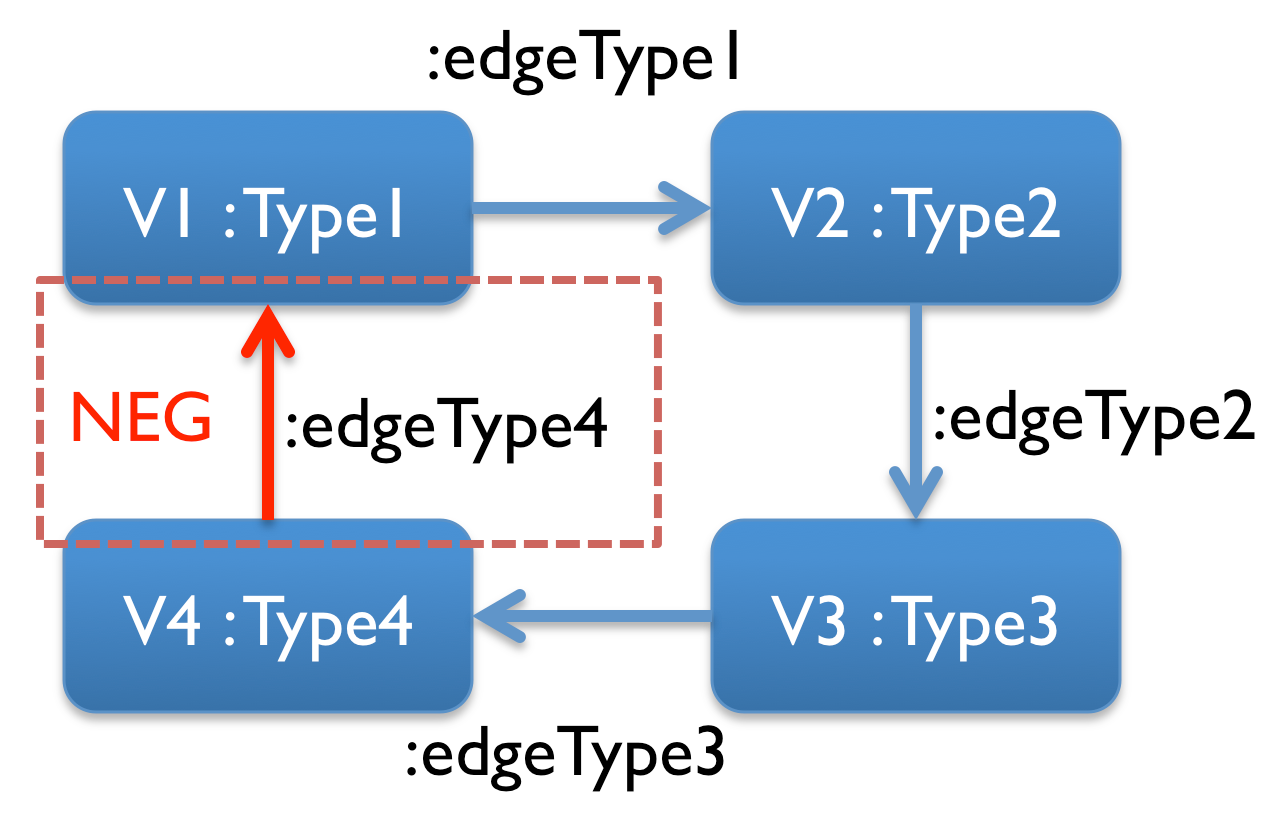
\includegraphics[width=\textwidth]{figures/patterndef}
\end{minipage}
\end{tabular}
\end{center}
\caption{Example graph query}
\label{fig:patterndef}
\end{figure}

\emph{Example.}
An example graph query is shown in \autoref{fig:patterndef} (the query is intentionally domain-independent to emphasize the generalizability of the approach), as a graph pattern definition in \incquery{} syntax~\cite{models10} on the left and graphically on the right. This query represents a typical pattern that is used in MDE applications (such as well-formedness validation or complex model transformations), whereby a subgraph of 4 connected vertices ($V1, V2, V3, V4$) is sought after with a \emph{negative application condition} prescribing that a typed edge (between vertices $V4$ and $V1$) must not exist.
The Rete network constructed for matching this graph pattern is depicted in \autoref{fig:retelayout}. In \incqueryD{}, type-instance indexers for edge types enumerate all source and target vertices, thus the intermediate join nodes perform join operations on vertex pairs that are connected by typed edges as prescribed by the definition in \autoref{fig:patterndef}. The join nodes all store the intermediate query results (e.g.\ connected $V1-V2$ and $V2-V3$ tuples in the case of the leftmost join node), and keep these caches up-to-date as change tokens arrive from the middleware (whenever model changes are performed).

\emph{Information representation and distributed operation.} The Rete layer of \incqueryD{} is \emph{domain and storage agnostic} as it stores only tuples constructed from model element identifiers and literals, thus it can be used independently of the model representation format (metamodeling language) of the model repository.
As illustrated in \autoref{fig:architecture}, the Rete nodes can be allocated to different hosts in a cloud computing infrastructure (as the communication protocol supports remoting). As change propagation is asynchronous, \incqueryD{} implements a \emph{termination protocol} to ensure that the query results can be retrieved consistently with the model state after a given transaction (i.e.\ by signaling when the update propagation has been terminated).

\begin{figure}[!tb]
\begin{center}
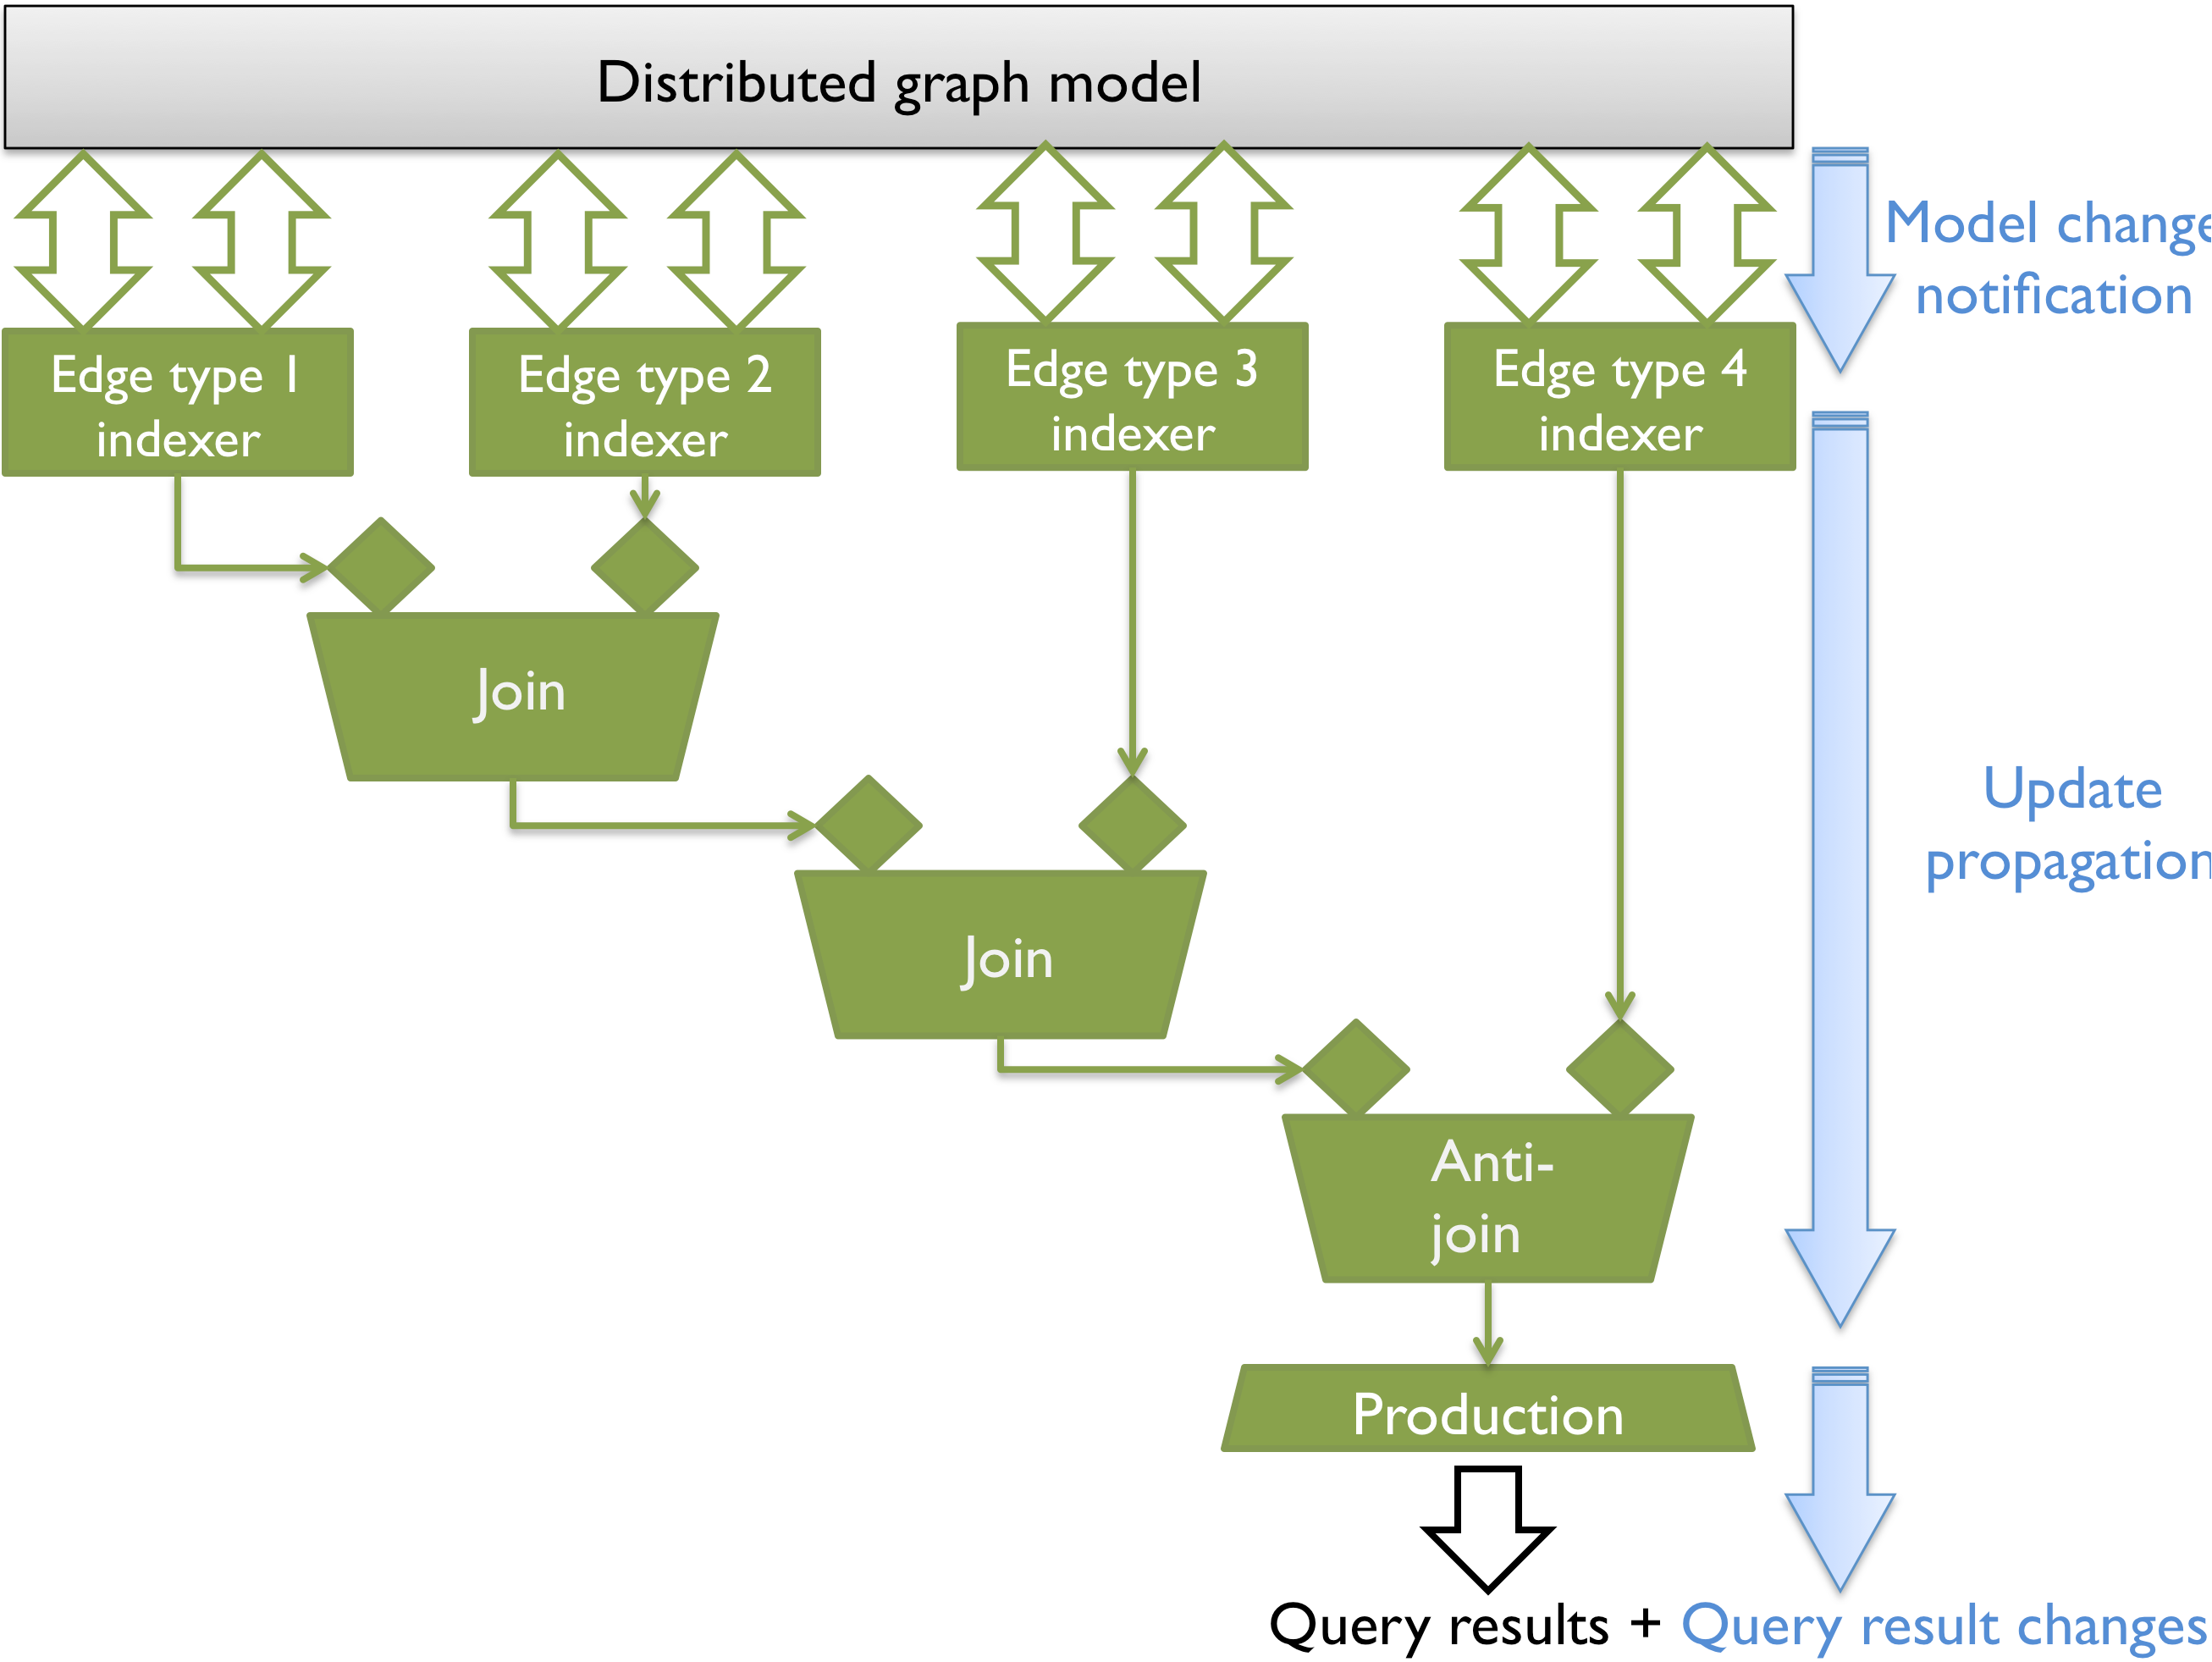
\includegraphics[width=.8\columnwidth]{figures/reteinternals}
\caption{Rete layout}
\label{fig:retelayout}
\end{center}
\end{figure}

\subsection{Scalability considerations}
For the storage layer, the most important issue from an incremental query evaluation perspective is that the indexers of the middleware should be filled as quickly as possible. This favors technologies where model sharding can be performed efficiently (i.e.\ with balanced shards in terms of type-instance relationships), and elementary queries (or model graph traversals) can be executed efficiently.

Achieving scalability of the distributed Rete architecture is an equally complex challenge. The overall performance of the system is influenced by a number of factors, including (i) the \emph{layout of the Rete network} (which can be optimized depending on both query and instance model characteristics, e.g.\ to keep the resource requirement of intermediate join operations to a minimum), (ii) the \emph{allocation} of Rete nodes to host computers (e.g.\ to optimize local resource usage, or to minimize the amount of remote network communication), and (iii) \emph{dynamic adaptability} to changing conditions (e.g.\ when the model size and thus query result size grows rapidly, the Rete network may require dynamic reallocation or node sharding due to local resource limitations).